Our architecture for implementing security metrics is straight forward. We declare a \textit{base security metric} type from which all metrics inherit three capabilities. Check Prerequisites: is invoked either directly by the caller or in the metric's own calculate method to ensure all items necessary for the calculation are present. Calculate: returns the resulting measurement. Get Metadata: returns the environment and ancillary data used during the calculation. 
% \end{itemize}

% \begin{figure}[ht]
% \centering
% 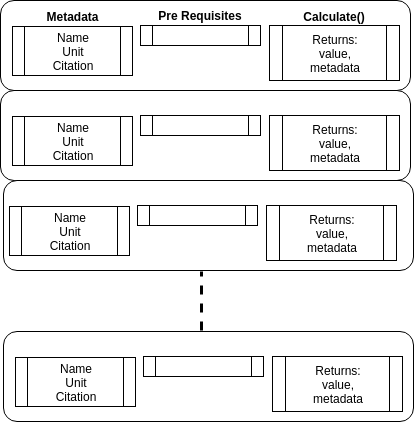
\includegraphics[width=.4\linewidth]{img/SecMet_archs.png}
% \caption{Security Metric Catalog (\textbf{SecMet})}
% \label{fig:automation:metric_arch}
% \end{figure} 

% As shown in Figure \ref{fig:automation:metric_arch}, 

This design allows us to implement a library of security metrics with a standard, stateless interface. We have been largely focused on attack graph based metrics, but tests against metrics using other structures (eg attack nets and economic/game theoretic models) suggests this architecture will support any type of security metric we've come across. Listing \ref{lst:secmet_flags} shows the runtime flags available to our library implementation. Because the derived system facts may change based on the rules asserted, after executing a test we can dump all primitive and derived facts to a JSON structure and use that to recreate the environment that produced a specific sample value. Because the original system is seldom referenced in attack graph metrics, we feel this is an important requirement not only for validating existing metrics, but also in developing more comprehensive, robust security measurements in the future. That is to say, there is a survivor-ship bias in attack graph based metrics, where the only systems that produce an attack graph are necessarily vulnerable between the selected start and end points. If a metric is exclusively operating on an attack graph for security measurement, then we have already determined the system is insecure and exploitable, and are only estimating the extent to which that system subgraph is resilient or susceptible given the current set of facts and interaction rules. 


% \begin{minipage}{.95\linewidth}
\begin{lstlisting}[language=Python, label={lst:secmet_flags}, caption={SecMet CLI Flags},captionpos=b,]]
secmet.metrics:
  --input_model_name: use this mulval model
  --secmet_ag_name: use this attack graph
  --secmet_ag_path: path to find attack graphs
  --secmet_fg_dot: fg dot file path (overrides path/name)
  --secmet_fg_name: use this fact graph
  --secmet_fg_path: path to find fact graphs
  --secmet_fix_cvss_score: Applies this cvss score to all vulnerabilities.
    (a number)
  --secmet_map_scores: Map AG scores to another domain
  --secmet_model_size: use exammpe models of this size
    (default: 'small')
  --secmet_model_type: use exaple models of this type
    (default: 'enterprise')
  --[no]secmet_plot_intermediate_graphs: Writes graphs to file when true.
    (default: 'false')
  --[no]secmet_random_cvss_score: Applies random cvss score to all
    vulnerabilities.
    (default: 'false')
  --secmet_random_seed: Use this seed for randoms
  --secmet_score_dict: use this score dictionary
  --secmet_score_strategy: Apply this weighting and scoring strategy
  \end{lstlisting}
% \end{minipage}

% \begin{table}[ht]
% \caption{Implemented Metrics}
% \resizebox{.45\textwidth}{!}{%
% \begin{tabular}{@{}lp{.35\linewidth}l@{}}
% \toprule
% Metric Class & Description & Common Measurements \\ \midrule
% Structural & Metrics based on the structure of the attack graph; used to identify attributes like shortest path, mean path length, or total number of paths. & SP, NP, MPL \\
% Time-Based & Metrics that quantify time expectations for attributes like compromise, recovery, or incident response. & MTTF, MTTB, MTTR \\
% Probability-Based & Metrics that associate probabilities attack paths to quantify the security of the network. & NR, PP, EPL \\
% Temporal & Metrics that examine  vulnerability age on the system. & TAG \\ \bottomrule
% \end{tabular}%
% }
% \label{tab:metric_summary}
% \end{table}


\begin{figure}[ht]
       \centering
        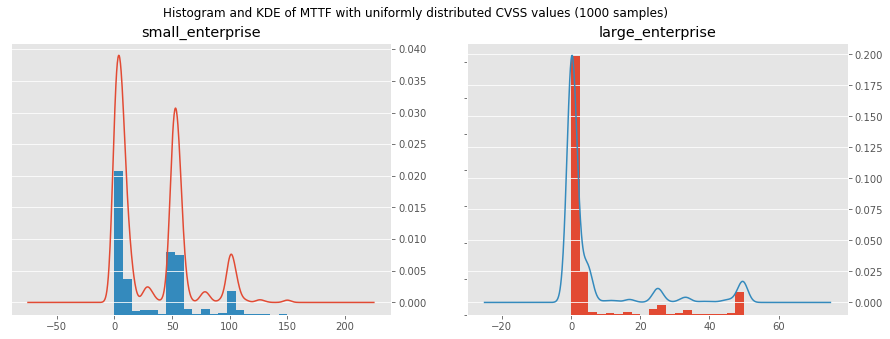
\includegraphics[width=\linewidth]{resource/img/ch_automation/from_ares_paper/hist_kde_svl.png} 
        \caption{MTTF distributions over 1000 random CVSS score assignments (uniform-dist)\cite{Dacier_1994}} 
        \label{fig:mttf_score_distributions}
\end{figure}

\begin{figure}[ht]
       \centering
        \includegraphics[width=\linewidth]{resource/img/ch_automation/from_ares_paper/fixed_100.png} 
        \caption{Fixing all vulnerability scores to determine lower and upper bounds for metric}     \label{fig:score_map_stepping}
\end{figure}




% \begin{figure*}
%       % \centering
%         \includegraphics[width=\linewidth]{img/analysis/fixed_100.png} 
%         \caption{Fixing all vulnerability scores to determine lower and upper bounds for metric}     \label{fig:result_density}
% \end{figure*} 


% \begin{figure*}
%     \centering
%     \begin{subfigure}[t]{0.3\textwidth}
%         % \centering
%         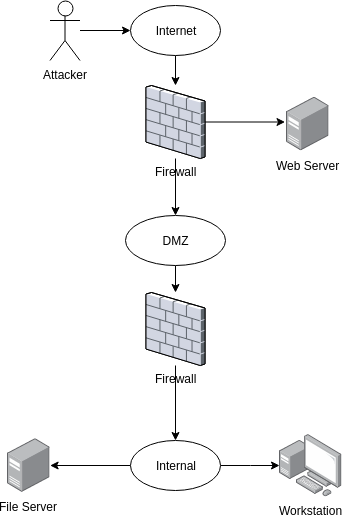
\includegraphics[width=\linewidth]{img/net_small.png} 
%         \caption{Small-sized network\cite{Ou_Appel_2005}} 
%         \label{fig:refnet_small}
%     \end{subfigure}
%           \begin{subfigure}[t]{0.3\textwidth}
%         \centering
%         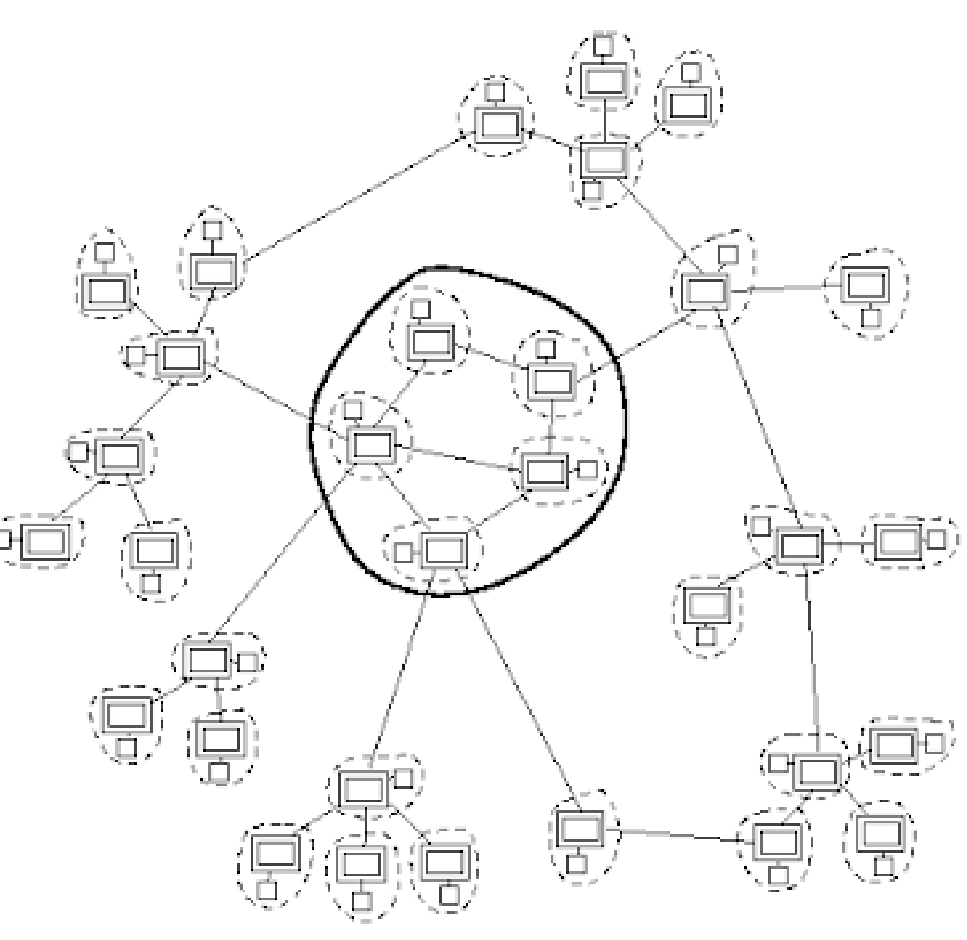
\includegraphics[width=\linewidth]{img/net_med_2.png}
%         \caption{Medium-sized network\cite{Cowie_Ogielski_Nicol_2002}}
%         \label{fig:refnet_med}
%     \end{subfigure}
%      \begin{subfigure}[t]{0.3\textwidth}
%         \centering
%         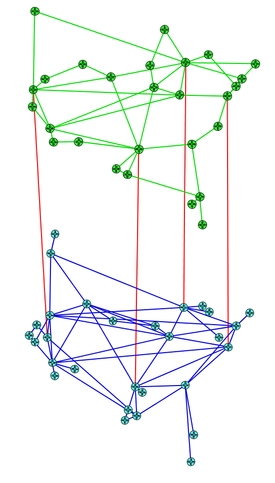
\includegraphics[width=\linewidth]{img/net_large.png}
%         \caption{Large-sized  network\cite{Cowie_Ogielski_Nicol_2002}}
%         \label{fig:refnet_large}
%     \end{subfigure}
%     \hfill
%     \caption{Different Sized Reference Networks}
%     \label{fig:refnets}
% \end{figure*}